% abthmsnp.tex
% Application-based TCP Hijacking
% Author: Oliver Zheng / Jason Poon / Konstantin Beznosov

\documentclass{sig-alternate}

% Drawing utilities
\input xy
\xyoption{all}

\begin{document}

% --- Metadata ---
\conferenceinfo{EuroSec}{'09 Nuremberg, Germany}
\CopyrightYear{2009}
%\crdata{0-12345-67-8/90/01}
% --- End Metadata ---

\title{
Application-Based TCP Hijacking
}

\numberofauthors {3}
\author {
	\alignauthor
	Oliver Zheng\\
		\email{eurosec@oliverzheng.com}
	\alignauthor
	Jason Poon\\
		\email{mr.j.poon@gmail.com}
	\alignauthor
	Konstantin Beznosov\\
		\email{beznosov@ece.ubc.ca}
}

\date{\today}

\maketitle

\begin{abstract}
We present application-based TCP hijacking (ABTH), a new attack on TCP applications that exploits flaws due to the interplay between TCP and application protocols to inject data into an application session without either server or client applications noticing the spoofing attack. 
Following the injection of a TCP packet, ABTH re-synchronizes the TCP stacks of both the server and the client.
To evaluate the feasibility and effectiveness of ABTH, we developed a tool that allows impersonating users of Windows Live Messenger in the matter of few seconds. 
Due to its generic nature, ABTH can be mounted on a variety of modern protocols for TCP-based applications.
Countermeasures to thwart and/or limit the effectiveness of ABTH could include strict Ethernet switching and cryptographic protection of messages. However, the former cannot be guaranteed by the application provider and the latter appears to be still prohibitively expensive for such large-scale applications with hundreds of millions of sporadic users as Windows Live Messenger.
\end{abstract}

\terms{Security, Theory}

\keywords{TCP hijacking, application-based TCP hijacking, Windows Live Messenger, application protocols, packet injection}

\section{Introduction}

Since its first specification in 1974~\cite{rfc:tcp}, the Transmission Control Protocol (TCP) has grown to become the core transport protocol for a vast number of applications including HTTP, FTP, SMTP, and TELNET.
The security properties of these application protocols are partially dependent on the security of TCP and the underlying Internet Protocol (IP).
Many network attacks that exploit vulnerabilities of the TCP design have shown prominence over the past decades~\cite{harris:tcpattacks}.
While preventive mechanisms have been developed to throttle or outright eliminate most of these attacks~\cite{dubrawsky:layer2}, the list of TCP vulnerabilities continues to grow.

In this paper, we present application-based TCP hijacking (ABTH), a new technique for attacking TCP-based communications.
ABTH extends TCP hijacking~\cite{stamp:infosec} by meddling with application-layer protocols.
Traditional TCP hijacking attacks exploit vulnerabilities of the transport and network layers.
However, the majority of these attacks have been circumvented through the use of hardware switches and routers~\cite{dubrawsky:layer2}, which provide countermeasures against such direct low-level attacks.
On the other hand, ABTH utilizes loopholes in the logistics of application-level communication to evade policy enforcement at the transport and IP layers.
Trivial design features of application protocols become fatal vulnerabilities that can be exploited by ABTH.

To demonstrate the feasibility and effectiveness of ABTH, a case study attacking the communications of Microsoft Windows Live Messenger (WLM) is presented.
With instant messaging (IM) becoming ubiquitous at both home and work~\cite{aol:survey}, WLM represents one of the largest IM networks.
By attacking the Microsoft Notification Protocol (MSNP)---the protocol in use by WLM---with ABTH, the privacy and confidentialiy of WLM users can be compromised; an attacker is capable of spoofing any command available to the WLM client and impersonating any contact known to the victim.
As a result, unauthorized messages can be delivered to various contacts.
We contacted Microsoft about the vulnerability of MSNP against ABTH in the spring of 2008.
As of September 2008, they were still ``looking at it.'' 
Although the reported case study is limited to WLM, due to its generic nature, ABTH can be mounted on a variety of application protocols.

Among several ways to circumvent ABTH, Internet service providers (ISPs) could employ stricter security controls on the network layer.
TCP applications could also employ TLS or other forms of data confidentiality and integrity protection.
However, the former cannot be guaranteed by the application provider(s) and the latter appears to be still prohibitively expensive for such large-scale applications with hundreds of millions of sporadic users as Windows Live Messenger.

The remainder of the paper is organized as follows.
Relevant background information on TCP and existing attacks on the transport protocol are discussed in Section~\ref{sec:background}.
The theory and general operation of ABTH is described in Section~\ref{sec:abth}.
The feasibility of ABTH for MSNP is demonstrated in Section~\ref{sec:casestudy}.
The limitations of ABTH and countermeasures against it are discussed in Section~\ref{sec:discussion}.
The paper is concluded in Section~\ref{sec:conclusion}.

\section{Background and Related Work}
\label{sec:background}

In this section, necessary background information on TCP including the details of existing security flaws are presented.

\subsection{Overview of TCP}

TCP is a connection-oriented transport protocol that guarantees reliable in-order delivery of network packets~\cite{rfc:tcp}.
A pair of hosts initiate contact and communicate by sending packets to each other.
Each end of the connection is identified by an Internet Protocol (IP) address and a TCP port, both of which are determined prior to the establishment of connection.

Each TCP packet is tagged with a sequence number, an acknowledgement number, and a receive window, herein referred to as seqnum, acknum, and rcvwnd, respectively.
seqnum represents the n-th byte of data transferred; acknum confirms the n-th byte of data received; rcvwnd corresponds to the number of bytes the host is willing to receive and capable of processing.
Within each TCP header are also 8 control bits or flags.
Packets containing data have the SYN and ACK flags set; packets with no data only have the ACK flag set to denote an empty acknowledgement packet.
For each data packet that is sent, an acknowledgement packet has to be received to affirm packet delivery.
A data packet with the same acknum may be received in lieu of an empty acknowledgement packet, in which case this packet needs confirmation as well.

In order for the two hosts to be in a synchronized state where data packets can be received and processed as valid packets, the seqnum of one host must match the acknum of the other and vice versa. 
As an example to illustrate seqnum and acknum, a client connects to a server through TCP.
After establishing a connection, assume the client has a seqnum of 50 and the server has a seqnum of 100.
The next packet the client sends must entail seqnum 50 and acknum 100.
If the client sends a data packet of 10 bytes, the client seqnum increases to 60 and the server must send an acknowledgement packet with seqnum 100 and acknum 60.

When either hosts receives a packet containing an unexpected seqnum two scenarios may occur.
If the received seqnum is within the range of the expected seqnum and the rcvwnd (the packet received arrived before another packet with the expected seqnum), the data is buffered and no acknowledgement packet is sent.
(An acknowledgement packet would confirm the reception of the missing packet.) Otherwise, the packet is dropped and an acknowledgement packet is sent with an acknum of the expected seqnum inciting a TCP ack storm~\cite{anderson:ackstorm} which is, in the persepective of an attacker, an undesirable effect.

\subsection{Adversary Model}
\label{sec:adversarymodel}

The main assumption about the adversary is that attackers are able to listen to network traffic of a TCP session and inject spoofed packets into the network.
We do not assume that the attacker has necessarily the capabilities of launching a denial-of-service attack, delete or reroute network traffic.
Sniffing and spoofing are limited in wired networks.
For example, network switches prevent sniffing in Ethernet and it is usually very hard to sniff on routers.
Internet service providers (ISPs) and enterprises often use network access control to block IP spoofing.
However, in wireless networks, especially in 802.11 networks, sniffing and spoofing can be done with well designed software and off-the-shelf hardware.
Computational capabilities of the attacker do not go beyond the limits of a consumer-level personal computer.
For example, in our implementation of of ABTH for Windows Live Messenger, the victim was attacked in the matter of two seconds with the use of a modest laptop.

\subsection{Attacks on TCP}

Many attacks on TCP exploit vulnerabilities of the seqnum and acknum synchronization mechanism.
In order to demonstrate the value of ABTH, attacks pertinent to ABTH are first discussed in the following sections.
All of these attacks, including ABTH, assume the threat model defined in Section~\ref{sec:adversarymodel}.

\subsubsection{TCP Hijacking}

By eavesdropping on a TCP session, an attacker is able to observe and calculate the expected seqnums and acknums of both hosts and is therefore able to inject a spoofed TCP packet~\cite{harris:tcpattacks}.
The spoofed packet would contain the seq and ack numbers expected by the recipient and the source address of the other host.
Although the spoofed packet is being sent by the attacker, the recipient does not have the ability to authenticate the source of the packet and would therefore accept it as a valid packet.
However, following this spoof, the connection is effectively broken as the expected seqnums and acknums of the two hosts are out of sync.
Data packets sent to either host would be regarded as invalid due to the mismatch of numbers, and no acknowledgement packets are sent in response.
Thus, the connection is quickly reset by both hosts.
As a result, both hosts would notice a disruption in the network service and may suspect an attack.

\subsubsection{Man-in-the-Middle}

Following a TCP hijacking attack, the attacker can act as the man-in-the-middle by relaying all messages from one host to the other~\cite{joncheray:simpleattack, gregg:stackhack}.
Although the initial spoofed packet has caused an imbalance between the TCP stacks of both hosts, for each packet sent by either hosts, an attacker is able to spoof an acknowledgement packet to the responding host by translating the seqnums and acknums on the fly.
However, a problem arises when each host receives the original packet(s) that was sent to each other.
As previously mentioned, a packet is considered valid if its seqnum falls within the range of the expected seqnum and the rcvwnd.
Spoofed packets cause the spoofed host to lag behind on its seqnum, and thus packets sent from the spoofed host are not in the acceptable range.
Subsequently, for each packet the spoofed host sends, the other host drops it and sends back an acknowledgement packet with the expected seqnum and acknum trying to correct this desynchronization.
The spoofed host would try to do the same by sending an acknowledgement packet, which incites the other host to send another.
This repeated cycle of sending packets creates an ack storm, in which both hosts continuously send empty ack packets.

While the ack storm stops as soon as one packet is dropped due to the unreliability of the underlying physical network, it creates a massive load of network traffic~\cite{joncheray:simpleattack}.
Intrusion detection systems can characterize this load with statistical analysis of empty packets on the network and notify users of the attack.

\subsubsection{ARP Poisoning}

A method of avoiding TCP ack storms is to stop hosts from receiving legitimate packets.
While the attacker cannot delete or reroute packets, the attacker can utilize Address Resolution Protocol (ARP) poisoning to mislead hosts into ignoring legitimate packets.
ARP provides translation of IP address to MAC address.
If the ARP is poisoned with the wrong MAC address, a host will send TCP/IP packets to the wrong MAC address and ignore incoming packets from the real MAC address.
The attacker needs only to ARP poison one host to circumvent ack storms, as the compromised host will not respond to the other host.

However, ARP traffic does not travel beyond the local area network (LAN) and imposes the restriction that the attacker be within the same LAN as at least one host.
More importantly, ARP poisoning is a low network level attack that can be easily prevented with hardware enforcement~\cite{spangler:sniffing}; most hardware switches disable ARP poisoning.

\subsubsection{Restoring Synchronization}

The attacker can try to resynchronize both hosts by inciting the lagging host to send packets manually~\cite{lam:resync}.
For example, an attacker exploiting the TELNET protocol may send a notice to the user to type in a few characters.
However, slightly more experienced users will easily detect such a peculiarity.

As discussed, existing attacks on TCP do not provide much guarantee for an attack to be executed unnoticed.

\section{Application-Based TCP Hijacking}
\label{sec:abth}

ABTH improves upon conventional TCP session hijacking by allowing an attacker to automatically resynchronize TCP seqnums and acknums of the two hosts of the connection.
It is a specific method of exercising TCP hijacking based on the application protocol without utilizing ARP poisoning or any other techniques below the transport layer.
The technique assumes the adversary model described in Section~\ref{sec:adversarymodel}. 
Computational capabilities of the attacker do not go beyond the limits of a consumer-level personal computer.
For example, in our implementation of ABTH for WLM, the victim was attacked in the matter of two seconds with the use of a modest laptop.

\subsection{Attack Details}

Many application protocols intended for two-way communication, such as TELNET and FTP, maintain a persistent TCP connection.
A typical method for ensuring the connection is open is for one of the hosts to periodically send a application-level command to the other host.
Application-level commands, such as a ping, feature two characteristics of particular importance: they prompt automatic response from the other host and they do not modify application states.

ABTH exploits these seemingly trivial application-level commands at the TCP level to perform TCP hijacking and resynchronization.
In most application protocols, a ping to a host will provoke a response; using this knowledge we can inflate the seqnum of the host.
Assuming ping responses exceed the data length of pings, by injecting certain multiples of pings directed at each host would counterbalance the difference created by an injected packet.

As a result, an attacker can spoof a packet containing a malicious command and is able to avoid an ack storm from occurring by spoofing multiple pings to the hosts to bring up a lagging seqnum of a host to a desired seqnum. 
The order in which these packets are injected should follow a specific rule.
For a packet sent by each host, the seqnum should fall within the acceptable range of the expected seqnum and rcvwnd, and the acknum should not be larger than the seqnum of the recipient host.
For the attacker, this means alternating the spoofing of packets between the two hosts for them to catch up to each other.
If followed correctly, only a few ack packets would be sent and no ack storm would ensue.

Once this is achieved, the connection is repaired and subsequent legitimate and/or illegitimate application commands can be received and processed successfully.
In comparison to typical TCP hijacking methods which usually lead victims suspicious of an attack, ABTH exploits a combination of TCP and the application protocol to execute an attack that conforms with the specification for TCP and the application protocol and also maintains a small network footprint.
Thus allowing the attacker to carry out an attack without using exploits prohibited and impractical in well-controlled networks and evading existing intrusion detection systems.
The significance of ABTH provides the attacker an exit strategy in which the attack may be executed unnoticed.

\section{Case Study: Windows Live Messenger}
\label{sec:casestudy}

First released in 1999, Windows Live Messenger (WLM) has since grown to become one of the most popular instant messaging (IM) services.
WLM uses the Microsoft Notification Protocol (MSNP) to communicate to servers within the .NET Messenger Service~\cite{piccard:imsecurity}.

\subsection{.NET Messenger Service}

The .Net Messenger Service provides WLM clients with instant messanging and presence services that are required for user-to-user communication.
As can be seen in Figure~\ref{fig:wlminfrastructure}, the service consists of a centralized cluster of servers; two types of servers exist within this cluster: notification servers (NS) and mixer servers~\cite{torre:wlm}.

\begin{figure}[h]
	\centering
	\caption{.NET Messenger Service Infrastructure}
	\label{fig:wlminfrastructure}
	\includegraphics{graphics/Infrastructure.eps}
\end{figure}

When a user logs into their WLM account, a persistent TCP connection to the NS is established.
This connection must always remain active for the lifetime of the session; a lost connection will result in the client being logged out and disconnected from the messaging service, which is reflected on the contact lists of the user's contacts.

Through the connection with the NS, control packets are transmitted to and from the user. 
Control packets include a user's contact list and presence information (e.g., user status, email notification).
The NS also sends information regarding mixer servers, which relays content packets between clients. 
Content packets consist of all messages sent between WLM clients through the mixer such as instant messages.
If user 1 attempts to talk to user 2, user 2 will receive from the connected NS the location of a mixer server, to which user 2 needs to connect in order to receive messages from user 1.

\subsection{Microsoft Notification Protocol}

\begin{table*}[tbp]
	\centering

	\caption {MSNP Commands}
	\label{tab:commandlist}

	\begin{tabular}{llr}
		\hline
		\hline
		\textbf{Command} & \textbf{Description} & \textbf{Size} \\
		\hline
		\texttt{PNG$\backslash$r$\backslash$n} & Client command to ping the NS. & 5 \\
		\texttt{QNG [2]$\backslash$r$\backslash$n} & NS's response to PNG. & 8 \\
		\texttt{CHL [22]$\backslash$r$\backslash$n} & NS command to ping the client. & 28 \\
		\texttt{QRY [24]$\backslash$r$\backslash$n[32]} & Client's response to CHL. & 60 \\
		\texttt{QRY [2]$\backslash$r$\backslash$n} & NS's response to client's QRY. & 8 \\
		\texttt{RNG [10] [ip:port] [19] [email] [name] [21] $\backslash$r$\backslash$n[ws]} & NS's invite to the client for new IM session. & 120 \\
		\hline
	\end{tabular}

	\begin{flushleft}
	Parts of commands are denoted using the following notation:

	\begin{itemize}
		\item {[\#]} is an integer or string of \# characters wide, irrelevant for the context of ABTH;
		\item {[ip:port]} is the IP address and TCP port of the mixer server;
		\item {[email]} is the email address of the user to be impersonated;
		\item {[name]} is the name of the user to be impersonated;
		\item {[ws]} is a variable length of whitespace padded to the command by the attacker.
	\end{itemize}
	\end{flushleft}
\end{table*}

MSNP is a text-based application protocol used for communication between WLM clients and servers.
Although the protocol was first intended to be an open standard~\cite{fout:insidewlm}, it has since become proprietary and has undergone numerous revisions.
However, due to the unencrypted nature of the protocol, attempts to reverse-engineer the protocol have proven successful~\cite{hypothetic:msnp, msnfanatic:msnp}.

The protocol consists of plain text commands; each MSNP command is prefixed with three capital letters (e.g., command \texttt{PNG} represents ping).

To determine the validity of the persistent connection between the NS and the client, MSNP allows for asynchronous bi-directional pings; both the WLM client and the NS have the ability to initiate a ping.
The client pings the NS with \texttt{PNG}; the NS pings the client with \texttt{CHL}.
Both pings provoke responses, which must be sent to prevent disconnection from the messaging service.
WLM, the official MSNP IM application, pings the NS every 45 seconds whereas in alternative IM clients such as Pidgin~\cite{pidgin:url}, ping the NS every 30 seconds.
Table~\ref{tab:commandlist} specifies the structure of those MSNP commands that are relevant to our ABTH attack on MSNP.
Note that the ping-response initiated by the NS entails three transactions (\texttt{CHL}-\texttt{QRY}-\texttt{QRY}).

An attacker can inject an MSNP command by listening to the TCP traffic.
Afterwards, ABTH can exploit these two sets of ping-response commands to eliminate the discrepancy between the seqnums and acknums of the client and the NS created by the spoof packet.
Completion of ABTH will circumvent disconnection and detection of a spoofed packet.
The fact that MSNP allows whitespace padding after commands allows for artificially inflated seqnums, simplifies ABTH calculations, and reduces the number of packets necessary to resynchronize the TCP connection.

In order to demonstrate the feasibility of ABTH, the follow section demonstrates the spoofing of an MSNP command without disconnecting the client.
The spoofed command creates the effect of identity impersonation.
The attack uses the official WLM client and the live .NET Messaging Service, as well as a a custom-made rogue WLM mixer server to which the WLM client connects.
Thus, scope of the attack is confined within the TCP connection between the NS and the user.

\subsection{Identity Spoofing}

When TCP seqnums are synchronized, NS acknum should match client seqnum and client acknum should match NS seqnum, as shown in the first row of Table~\ref{tab:identityspoof}.
An attacker can inject a \texttt{RNG} command to the client, who will open a new TCP connection and connect to the address of a mixer server (which the attacker may specify as a rogue mixer).
Following the injection of the packet, the seqnums and acknums of the WLM client and the NS become desynchronized and can be resynchronized with ABTH.
For demonstration purposes, the seqnums of the client and the NS are assumed to be 100 and 500 prior to the spoofed packet.

While the seqnums of the NS or the client cannot be controlled, pings can provoke responses to inflate seqnums.
Each command is sent or received by the attacker in the order listed in Table~\ref{tab:identityspoof}.

\begin{table*}[tbp]
	\centering

	\caption{Identity Spoofing Sequence Numbers}
	\label{tab:identityspoof}

	\begin{tabular}{l l l r r r r r}
		\hline
		\hline
		\textbf{Command} & \textbf{Sent By} & \textbf{Received By} & \textbf{Data Size} & \textbf{Client Seq} & \textbf{Client Ack} & \textbf{NS Seq} & \textbf{NS Ack} \\
		\hline
		\multicolumn{4}{l}{\textbf{Before Attack}} & 100 & 500 & 500 & 100 \\
		RNG & Attacker & Client & 120 & 100 & \textbf{620} & 500 & 100 \\
		\multicolumn{8}{l}{\textbf{Begin ABTH}} \\
		PNG & Attacker & NS & 5 & 100 & 620 & 500 & \textbf{105} \\
		QNG & NS & Attacker & 8 & 100 & 620 & \textbf{508} & 105 \\
		\multicolumn{4}{l}{\textbf{Repeat PNG/QNG exchange for 23 more times}} & 100 & 620 & \textbf{692} & \textbf{220} \\
		CHL & Attacker & Client & 28 & 100 & \textbf{648} & 692 & 220 \\
		QRY & Client & Attacker & 60 & \textbf{160} & 648 & 692 & 220 \\
		QRY & Attacker & Client & 8 & 160 & \textbf{656} & 692 & 220 \\
		CHL & Attacker & Client & 28 & 100 & \textbf{684} & 692 & 220 \\
		QRY & Client & Attacker & 60 & \textbf{220} & 684 & 692 & 220 \\
		QRY & Attacker & Client & 8 & 220 & \textbf{692} & 692 & 220 \\
		\hline
		\hline
		\multicolumn{4}{l}{\textbf{After ABTH}} & 220 & 692 & 692 & 220 \\
	\end{tabular}
\end{table*}

As the last row of Table~\ref{tab:identityspoof} shows, with matching seqnums and acknums, ABTH has successfully completed its series of application specific commands and resynchronized and the TCP connection.
The connection is now is ready to transmit further legitimate and/or illegitimate packets.

At this point, the victim will have established a connection to the rogue mixer server, which acts as a regular server that can send and receive messages as any user the attacker wishes to impersonate.
The victim would not recognize such imposture, as the victim cannot differentiate a rogue mixer server from a legitimate one.
No additional attacks are required to send and receive any message from the victim as the impersonated user.

\section{Discussion}
\label{sec:discussion}

Our experiments demonstrate that MSNP can be successfully attacked by through ABTH.
However, ABTH has several caveats.

\subsection{Limitations}

In the case with WLM, it is crucial that ABTH is completed prior to the next client ping, which occurs in roughly 45 seconds.
Otherwise, the client would repeatedly ping the NS and discover the imbalance in seqnums, eventually leading to a timeout and disconnection.
Depending on the resources of the attacker, ABTH can be reasonably accomplished within this timeframe, as our experiments demonstrated, later described in the feasibility section.

ABTH requires the length of responses be greater than the commands issued to provoke them.
If this was not the case, resynchronization would only widen the gap of mismatched seqnums.
Likewise, application commands with similar behaviour to NOP (no operation) that do not provoke responses would not work either.

Our implementation of ABTH on the MSNP protocol calculates and generates the required commands to send prior to the attack and are therefore static.
If either host sends packets during the restoration phase, this would result in ABTH to fail in resynchronizing their TCP stacks.
As a result, no network traffic can occur while ABTH is in the process of sending its own packets.
Complex algorithms capable of adjusting to live traffic dynamically may improve this performance.

\subsection{Countermeasures}

In order to properly authenticate messages, a straight-forward countermeasure against ABTH is to encrypt all application traffic, for example with SSL/TLS.
However, with over 17 million unique user~\cite{templeton:spoof}, WLM and other large-scale applications would require substantial server resources to encrypt all network traffic.
In the scenario where applications connect peers to peers by allowing a communication channel between two clients, as MSNP implicitly does through the mixer connection, clients may encrypt traffic and authenticate each other through the channel provided by the application.
As a case in point, SimpLite-MSN~\cite{secway:url} sets up RSA keys and authenticates all instant messaging traffic for MSNP, thus providing protection against spoofing.

As ABTH requires a predetermined number of spoof packets to inflate the seqnums and acknums of the hosts, intrusion detection systems (IDS) may detect this form of attack due to the sudden spike in traffic between the hosts.
However, this behaviour may step within the boundaries of legitimate application traffic.

Furthermore, a regulatory mechanism in the application protocol, such as tagging application messages with sequence numbers, has the potential for providing integrity for each packet.
With such a mechanism, it would be difficult to inject a packet and expect further messages to be accepted as the application keeps track of the list of messages.
This straightforward yet non-trivial detail also alleviates the application protocol from its dependence on the network layer and the assumption that packets on the network layer are authentic.

For network service providers, the most effective method to disable ABTH and message spoofing all together would be to prohibit IP packets with forged source IP addresses~\cite{templeton:spoof}.
However, this method would be ineffective in a wireless medium, such as WiFi.

\subsection{Feasibility}

Our particular implementation of ABTH on MSNP completes within roughly 2 seconds and is triggered on the reception of a MSNP \texttt{PNG} command.
In order for the attack to succeed, no network traffic can occur within these 2 seconds.
Although the amount of MSNP traffic varies depending on the time of day, number of contacts, and other factors, the logs obtained through monitoring several days of network traffic have concluded that probability of network traffic occurring within 2 seconds of a ping is less than 5\%, as shown in Figure~\ref{fig:successrate}.
With the statistics we have gathered, it seems that success rate of an ABTH attack has no relevance to the number of contacts online and thus the amount of network traffic.
(This could be due to the fact that \texttt{PNG}s are not sent until after 45 seconds of network inactivity, at which point the amount of network traffic has very little influence.)
As such, ABTH would prevail over 95\% of the time, a large concern for potential threat.

\begin{figure}[h]
	\centering
	\caption{Success Rate of ABTH attack vs the number of contacts online.}
	\label{fig:successrate}
	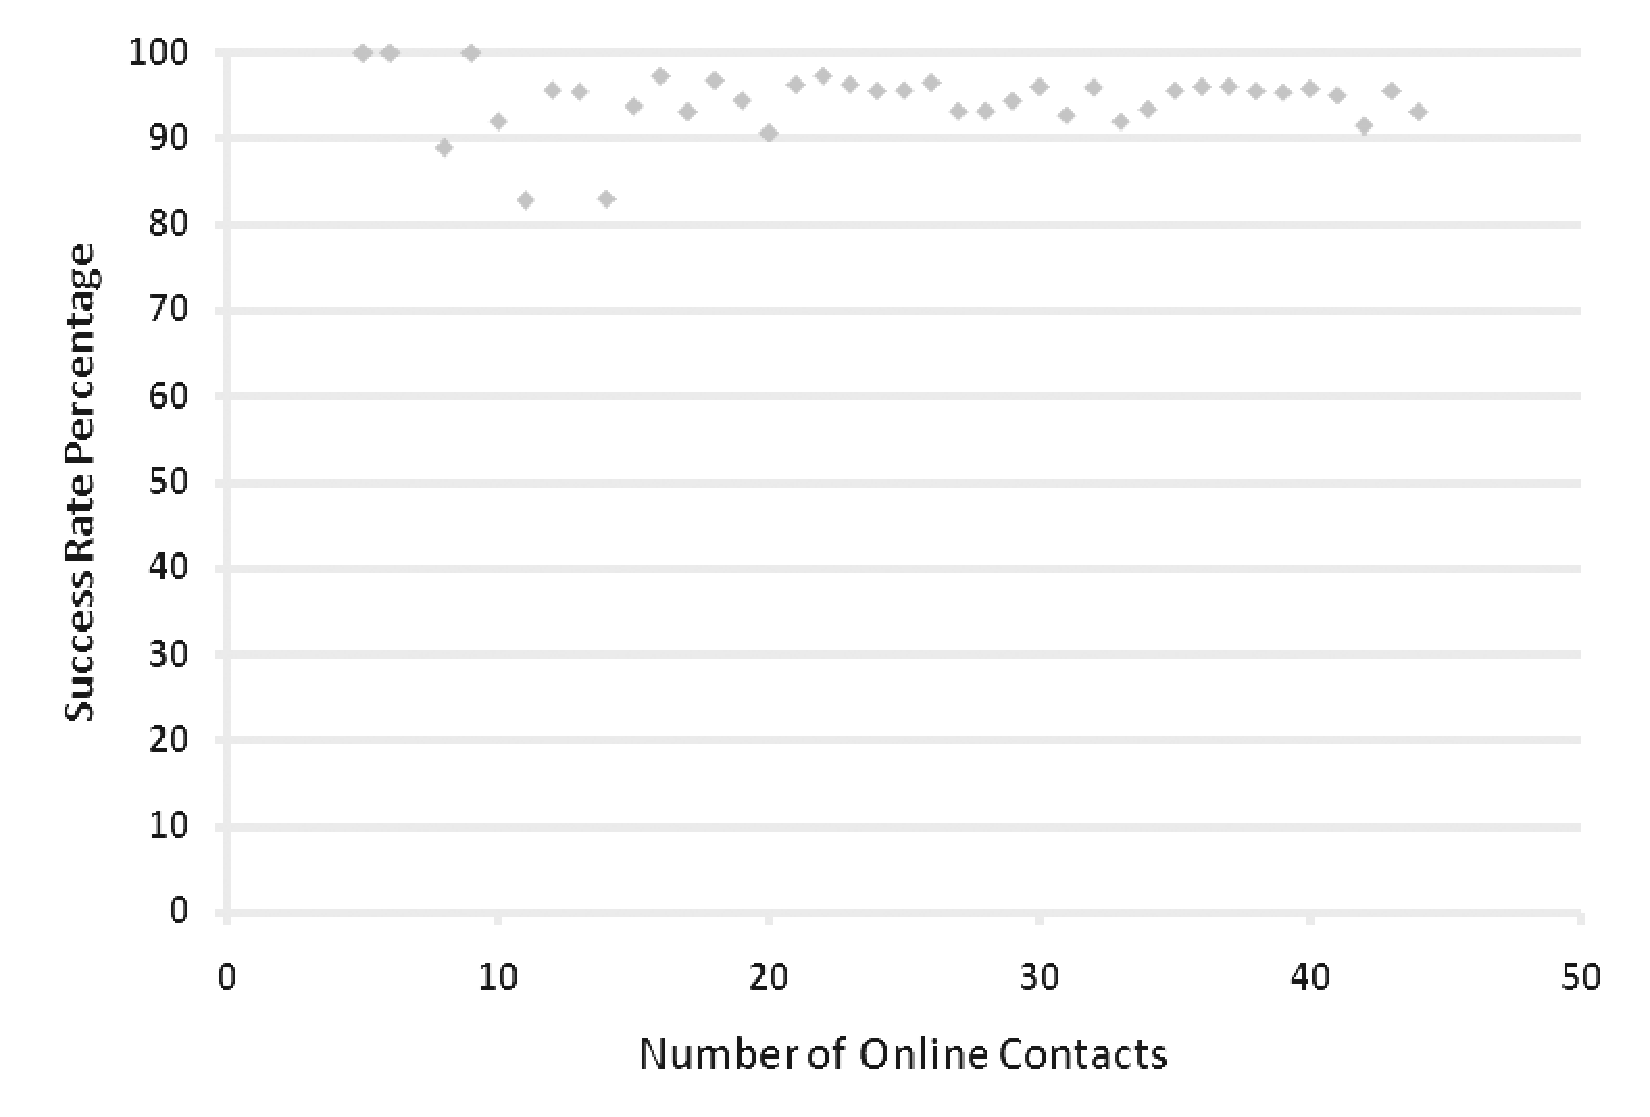
\includegraphics[width=\columnwidth]{graphics/plot.eps}
\end{figure}

In environments that provide a common physical communication medium, such as hubbed networks and coffee shops that offer WiFi service, ABTH poses a threat.
Application protocols vulnerable to ABTH, such as MSNP, were not designed to offer secure communication channels.
As such, it is imperative that, as protocols become more widely adopted, they are improved upon and revised to accommodate their broadening uses.

\section{Conclusion}
\label{sec:conclusion}

By combining the innocuous features of the transport and application layers and the lack of cryptographic protection at either layer, Application-Based TCP Hijacking (ABTH) offers a clean way of exploiting certain application protocols.
Sending commands to both hosts to provoke responses allows an attacker to create a gap in TCP sequence numbers of a size exactly large enough for the injection of a malicious command.
We presented a proof of the ABTH concept by successfully evaluating it against Windows Live Messenger, Microsoft's popular instant messaging application, which uses the Microsoft Notification Protocol (MSNP).

While some protocols, such as MSNP, were designed to suit flexible environments, as the environment evolved, these features have become subtle vulnerabilities.
Although hardware Ethernet equipment has been updated to obstruct lower level attacks (e.g., ARP poisoning), the realm of attacks is reaching beyond the protection capabilities of network devices.

\bibliographystyle{abbrv}
\bibliography{abthmsnp}

\end{document}
